\documentclass[dvipdfmx,a4paper,11pt]{article}
\usepackage[utf8]{inputenc}
%\usepackage[dvipdfmx]{hyperref} %リンクを有効にする
\usepackage{url} %同上
\usepackage{amsmath,amssymb} %もちろん
\usepackage{amsfonts,amsthm,mathtools} %もちろん
\usepackage{braket,physics} %あると便利なやつ
\usepackage{bm} %ラプラシアンで使った
\usepackage[top=30truemm,bottom=30truemm,left=25truemm,right=25truemm]{geometry} %余白設定
\usepackage{latexsym} %ごくたまに必要になる
\renewcommand{\kanjifamilydefault}{\gtdefault}
\usepackage{otf} %宗教上の理由でmin10が嫌いなので


\usepackage[all]{xy}
\usepackage{amsthm,amsmath,amssymb,comment}
\usepackage{amsmath}    % \UTF{00E6}\UTF{0095}°\UTF{00E5}\UTF{00AD}\UTF{00A6}\UTF{00E7}\UTF{0094}¨
\usepackage{amssymb}  
\usepackage{color}
\usepackage{amscd}
\usepackage{amsthm}  
\usepackage{wrapfig}
\usepackage{comment}	
\usepackage{graphicx}
\usepackage{setspace}
\usepackage{pxrubrica}
\usepackage{enumitem}
\usepackage{mathrsfs} 
\usepackage[dvipdfmx]{hyperref}
\setstretch{1.2}


\newcommand{\R}{\mathbb{R}}
\newcommand{\Z}{\mathbb{Z}}
\newcommand{\Q}{\mathbb{Q}} 
\newcommand{\N}{\mathbb{N}}
\newcommand{\C}{\mathbb{C}} 
\newcommand{\Sin}{\text{Sin}^{-1}} 
\newcommand{\Cos}{\text{Cos}^{-1}} 
\newcommand{\Tan}{\text{Tan}^{-1}} 
\newcommand{\invsin}{\text{Sin}^{-1}} 
\newcommand{\invcos}{\text{Cos}^{-1}} 
\newcommand{\invtan}{\text{Tan}^{-1}} 
\newcommand{\Area}{S}
\newcommand{\vol}{\text{Vol}}
\newcommand{\maru}[1]{\raise0.2ex\hbox{\textcircled{\tiny{#1}}}}
\newcommand{\sgn}{{\rm sgn}}
%\newcommand{\rank}{{\rm rank}}



   %当然のようにやる.
\allowdisplaybreaks[4]
   %もちろん.
%\title{第1回. 多変数の連続写像 (岩井雅崇, 2020/10/06)}
%\author{岩井雅崇}
%\date{2020/10/06}
%ここまで今回の記事関係ない
\usepackage{tcolorbox}
\tcbuselibrary{breakable, skins, theorems}

\theoremstyle{definition}
\newtheorem{thm}{定理}
\newtheorem{lem}[thm]{補題}
\newtheorem{prop}[thm]{命題}
\newtheorem{cor}[thm]{系}
\newtheorem{claim}[thm]{主張}
\newtheorem{dfn}[thm]{定義}
\newtheorem{rem}[thm]{注意}
\newtheorem{exa}[thm]{例}
\newtheorem{conj}[thm]{予想}
\newtheorem{prob}[thm]{問題}
\newtheorem{rema}[thm]{補足}
\newtheorem{dfnthm}[thm]{定義・定理}

\DeclareMathOperator{\Ric}{Ric}
\DeclareMathOperator{\Vol}{Vol}
 \newcommand{\pdrv}[2]{\frac{\partial #1}{\partial #2}}
 \newcommand{\drv}[2]{\frac{d #1}{d#2}}
  \newcommand{\ppdrv}[3]{\frac{\partial #1}{\partial #2 \partial #3}}

\title{基礎解析学2 -一変数と多変数の積分-}
\author{岩井雅崇 (大阪大学)}
\date{\today \, ver 1.00}
%ここから本文.
\begin{document}

\maketitle
\tableofcontents

\section{一変数の積分}

\subsection{微分積分学の基本定理 (三宅先生の本, 3.1と3.4の内容)}
\label{kihonteiri}

 この回の内容はかなり難しいので, 積分の理論を気にせず計算だけしたい人はこの回の内容を読み飛ばして, \ref{1_2}節の内容に移って良い.
 %(最後の誤差評価は使えるかもしれませんが...)
 また証明等を少々省略するので, 詳しくリーマン積分を理解したい人は「杉浦光夫 解析入門 1 (東京大学出版会)」を見てほしい.
% \begin{itemize}\item 杉浦光夫 解析入門 1 (東京大学出版会)\end{itemize}
 
%動画冒頭に述べたルベーグ積分を理解したい人は次の文献を見てほしい.(めちゃくちゃ難しいですが...) \begin{itemize} \item 伊藤清三 ルベーグ積分入門 (裳華房) \item Terence Tao \textit{An introduction to measure theory} available at \url{https://terrytao.files.wordpress.com/2011/01/measure-book1.pdf} \end{itemize}リーマン積分もルベーグ積分もどちらも計算上は違いはないので, 積分の理論を気にせず, 計算だけしたい場合は気にしなくて良いです.


\subsubsection{リーマン積分の定義}
この節では$I = [a,b]$とし, $f(x)$は$I$上の関数とする.
 \begin{itemize}
 
  \item \underline{関数$f(x)$が$I$上で有界}であるとは, ある正の数$M>0$があって, 任意の$x \in I$について$|f(x) |<M$となること.\footnote{$I$上で連続ならば$f(x)$は有界なので, わからなければ$f(x)$は連続として良いです.}
  
\hspace{-22pt} 以下, 関数$f(x)$が$I$上で有界であるとする.
 \item \underline{$\Delta$が$I$の分割}とは, 正の自然数$m$と
 $
 a = x_{0}<x_1< \dots <x_{m-1}<x_{m}=b %\text{\,\,となる}
 $
となる数の組$( a, x_1, \dots , x_{m-1} , b) $のこと.
 以下$\Delta = ( a, x_1, \dots , x_{m-1} , b ) $とかく. (この授業だけの記号である.)
 \item $\Delta$を$I$の分割として, \underline{$\Delta$の幅}を
 $
| \Delta| = \max_{1 \leqq i \leqq m} \{ |x_i - x_{i-1}| \} 
 \text{\,\,とする.}
 $
 
 \item $\Delta$を$I$の分割とする.
 $1 \leqq i \leqq m$となる自然数$i$について
 $$
 M_{i} = \sup \{ f(x) \,\,| \,\,x_{i-1} \leqq x \leqq x_i \}, \text{\,\,\,\,}
 m_{i} = \inf \{ f(x) \,\,| \,\,x_{i-1} \leqq x \leqq x_i  \} \text{\,\,とし, }
$$
 $$
 S_{\Delta} = \sum_{i=1}^{m} M_{i}(x_i - x_{i-1}), \text{\,\,\,\,}
  T_{\Delta} =\sum_{i=1}^{m} m_{i}(x_i - x_{i-1})\text{\,\,とおく. }
 $$
定義から$T_{\Delta} \leqq S_{\Delta}$となる.

 \end{itemize}
 
  \begin{tcolorbox}[
    colback = white,
    colframe = green!35!black,
    fonttitle = \bfseries,
    breakable = true]
    \begin{thm}[ダルブーの定理]
    ある実数$S,T$があって, 
    $$
    \lim_{|\Delta| \rightarrow 0}S_{\Delta} = S, \text{\,\,} \lim_{|\Delta| \rightarrow 0}T_{\Delta} = T.
    $$
    \end{thm}
    \end{tcolorbox}
    \footnote{$\lim_{|\Delta| \rightarrow 0}S_{\Delta} = S$の意味は, $\Delta$の幅が0になるように分割をとっていくと, $S_{\Delta}$は$S$に限りなく近くという意味である.}
    
      \begin{tcolorbox}[
    colback = white,
    colframe = green!35!black,
    fonttitle = \bfseries,
    breakable = true]
    \begin{dfn}[リーマン積分の定義]
    $I = [a,b]$かつ$f(x)$を$I$上の有界関数とする. \\
    \underline{$f$が$I$上でリーマン積分可能(リーマン可積分)}とは$S=T$となること.
    このとき, 
    $$
    S = \int_{a}^{b} f(x)dx \text{\,\,と表す.}
    $$
    \underline{$\int_{a}^{b} f(x)dx $を$f(x)$の$[a,b]$における定積分}という.
    
    また
    $$
    \int_{a}^{a} f(x)dx  =0, \text{\,\,\,\,} \int_{b}^{a} f(x)dx = -\int_{a}^{b} f(x)dx 
    \text{\,\,とする.}$$
    \end{dfn}
    \end{tcolorbox}
    以下, リーマン積分可能を単に積分可能ということにする.

\begin{exa}
\label{riem_not}
\begin{itemize}
\item $I = [a,b]$とし, $f$を$I$上での連続関数とする.
このとき$f$は$I$上で積分可能.(みんながよく知っている関数は積分可能.)
\item $I = [0,1]$とし, $I$上の有界関数$f(x)$を
$$
  f(x)= \begin{cases}
     1& \text{$x$は有理数}\\
    0& \text{$x$は無理数}
  \end{cases}
$$
とおくとき, 任意の$I$の分割$\Delta$について, $S_{\Delta}=1$であり, $T_{\Delta}=0$である.
よって$S =1$かつ$T=0$より, $f$は$I$上で積分可能ではない.
%\footnote{ルベーグ積分は可能になる. 積分値は0となる. ルベーグ積分はいい感じにリーマン積分を包含する概念である.}
 \end{itemize}
\end{exa}

      \begin{tcolorbox}[
    colback = white,
    colframe = green!35!black,
    fonttitle = \bfseries,
    breakable = true]
    \begin{thm}[区分求積法]
$I=[a,b]$とし, $f(x)$を$I$上の積分可能な関数とする.
任意の$n\in N$について, 
$x_i = a + \frac{(b-a)i}{n}$
($i$は$1 \leqq i \leqq n$なる自然数)とおき, 
$
D_n = \sum_{i=1}^{n} \frac{f(x_i)}{n} %\text{\,\,\ とすると}
$
とすると, 
$$
 \lim_{n \rightarrow \infty }D_n = \int_{a}^{b} f(x) dx\text{\,\,\ となる.}
$$
        \end{thm}
    \end{tcolorbox}
 \begin{exa}
 $I =[0,1]$とし, $f(x) =x^2$を$I$上の関数とする.
 任意の$n\in N$について, 
$x_i = 0+ \frac{(1-0)i}{n} = \frac{i}{n}$($i$は$1 \leqq i \leqq n$なる自然数)であるので, 
$$
D_n =  \sum_{i=1}^{n} \frac{f(x_i)}{n} 
= \sum_{i=1}^{n} \frac{i^2}{n^3} = \frac{n(n+1)(2n+1)}{6n^3}
$$
以上より区分求積法から
$$
\int_{0}^{1} x^2 dx =
 \lim_{n \rightarrow \infty }D_n = \frac{1}{3}\text{\,\,\ である.}
$$
 \end{exa}

    
\subsubsection{微分積分学の基本定理}

      \begin{tcolorbox}[
    colback = white,
    colframe = green!35!black,
    fonttitle = \bfseries,
    breakable = true]
    \begin{dfn}
    $f(x)$を区間$I$上の連続関数とする.
    $a \in I$を一つ固定する.
     $$
\begin{array}{cccc}
F: &I& \rightarrow & \R  \\
&x& \longmapsto & \int_{a}^{x} f(x) dx
\end{array}
$$
を\underline{$f(x)$の不定積分}と呼ぶ. 
\underline{$F(x)$を$\int f(x) dx$とも表す.}
不定積分は定数を除いてただ一つに定まる.
        \end{dfn}
    \end{tcolorbox}
      \begin{tcolorbox}[
    colback = white,
    colframe = green!35!black,
    fonttitle = \bfseries,
    breakable = true]
    \begin{thm}[微分積分学の基本定理]
    $f(x)$を区間$I$上の連続関数とする.
不定積分$F(x) = \int_{a}^{x} f(x) dx$は$I$上で微分可能で
$F'(x)=f(x)$である.特に
$$
\drv{}{x} \int_{a}^{x} f(t)dt = f(x) \text{\,\,\,である.}
$$
        \end{thm}
    \end{tcolorbox}
    
\begin{tcolorbox}[
    colback = white,
    colframe = green!35!black,
    fonttitle = \bfseries,
    breakable = true]
    \begin{prop}
    $f(x)$を区間$I$上の連続関数とし, $G(x)$を$I$上の関数とする.
    $G'(x) = f(x)$ならばある定数$c$があって, 
    $$
    G(x) = \int f(x) dx + c \text{\,\,\,となる.}
    $$
        \end{prop}
    \end{tcolorbox}
\begin{exa}
$f(x) = x^2, G(x) = \frac{x^3}{3}$とすると
$G'(x) = \left( \frac{x^3}{3} \right)' = x^2=f(x)$よりある定数$c$があって
$ \int x^2 dx   = \frac{x^3}{3} + c$となる.

\end{exa}
    
 
\begin{tcolorbox}[
    colback = white,
    colframe = green!35!black,
    fonttitle = \bfseries,
    breakable = true]
    \begin{thm}
    $f(x)$を$[a,b]$上の連続関数とし, $G(x)$を$G'(x) = f(x)$となる$[a,b]$上の関数とする.
このとき
$$
\int_{a}^{b} f(x) dx = \Bigl[ G(x) \Bigr]_{a}^{b} = G(b) - G(a) \text{\,\,\,となる.}
$$
        \end{thm}
    \end{tcolorbox}

\begin{exa}
$$\int^{1}_{0} x^2 dx = \left[\frac{x^3}{3}\right]^{1}_{0} =\frac{1}{3} $$である.
(区分求積法を用いるよりもずっとずっと簡単である.)
\end{exa}
    
 
\subsection{積分の性質 (三宅先生の本, 3.1と3.2の内容)}
\label{1_2}

\subsubsection{積分の性質}
 
 \begin{comment}


\begin{tcolorbox}[
    colback = white,
    colframe = green!35!black,
    fonttitle = \bfseries,
    breakable = true]
    \begin{thm}
    $f(x)$を$[a,b]$上の連続関数とし, $F(x)$を$F'(x) = f(x)$となる$[a,b]$上の関数とする.
このとき
$$
\int_{a}^{b} f(x) dx = \Bigl[ F(x) \Bigr]_{a}^{b} = F(b) - F(a) \text{\,\,\,となる.}
$$
        \end{thm}
    \end{tcolorbox}
    
  \end{comment}
  
  
    \begin{tcolorbox}[
    colback = white,
    colframe = green!35!black,
    fonttitle = \bfseries,
    breakable = true]
    \begin{prop}[積分の性質]
$f(x), g(x)$共に$[a,b]$上の連続関数とし, $G(x) = \int g(x) dx$とする.
\begin{enumerate}
    \setlength{\parskip}{0cm} 
  \setlength{\itemsep}{0cm} 
\item $\int_{a}^{b} (f(x) \pm g(x)) dx = \int_{a}^{b} f(x) dx \pm \int_{a}^{b} g(x) dx$
\item $k$を定数とするとき, $\int_{a}^{b} kf(x) dx  = k \int_{a}^{b} f(x) dx $
\item (置換積分法)    $$
\begin{array}{cccc}
x(t): &[\alpha, \beta]& \rightarrow & [a,b]\\
&t& \longmapsto & x(t)
\end{array}
$$
を$C^1$級関数とし, $a = x(\alpha), b=x(\beta)$とするとき
$$
\int_{a}^{b} f(x) dx = \int_{\alpha}^{\beta} f(x(t)) \drv{x(t)}{t} dt \text{\,\,\,となる.}
$$
\item (部分積分法)  $f(x)$が$C^1$級であるとき,
$$
\int_{a}^{b} f(x) g(x)dx = \Bigl[ f(x) G(x)\Bigr]^{b}_{a} - \int_{a}^{b}f'(x) G(x)dx
\text{\,\,\,となる.}$$
\end{enumerate}

        \end{prop}
    \end{tcolorbox}

\subsubsection{不定積分の例}
簡単な積分に関してまとめておく. %(以下は覚えなくても良い.) 
積分定数に関しては省略する. また$a$を実数とする.
  \begin{align*}
\begin{split}
\int x^a \,dx &= \frac{x^{a+1}}{a+1} \text{\,\,\, ($a \neq -1$のとき)}\\
\int \frac{1}{x} \,dx &= \log |x|\\
\int \frac{1}{\sqrt{a^2 - x^2}} \,dx &= \Sin \frac{x}{|a|} \text{\,\,\, ($a \neq 0$のとき)}\\
\int \frac{1}{a^2 + x^2} \,dx &= \frac{1}{a}\Tan \frac{x}{a} \text{\,\,\, ($a \neq 0$のとき)}\\
\int e^x \,dx &=e^x\\
\int a^x \,dx &=\frac{1}{\log a}a^x \text{\,\,\, ($a>0$かつ$a \neq 1$のとき)} \\
\int \log x  \,dx &=x \log x -x\\
\int \sin x  \,dx &=-\cos x \\
\int \cos x  \,dx &=\sin x \\
\int \frac{1}{(\cos x)^2}  \,dx &=\tan x \\
\end{split}
\end{align*}
 
 %%%%%%%%%%%%%%%%%%%%
 \begin{comment}


\subsubsection{ウォリスの公式}

\begin{tcolorbox}[
    colback = white,
    colframe = green!35!black,
    fonttitle = \bfseries,
    breakable = true]
    \begin{thm}
 $n$を自然数として, 
 $$I_n = \int_{0}^{\frac{\pi}{2}} (\cos t)^n dt =\int_{0}^{\frac{\pi}{2}} (\sin t)^n dt \text{\,\,とする.}$$
$n$が偶数のとき, 
$$
 I_n =  
 \frac{(n-1)!!}{n!!}\frac{\pi}{2} 
 =
 \frac{n-1}{n}\cdot\frac{n-3}{n-2} \cdots \frac{3}{4}\cdot\frac{1}{2}\cdot \frac{\pi}{2}\text{\,\,であり.}
$$
$n$が奇数のとき, 
$$
 I_n =  \frac{(n-1)!!}{n!!} 
 =
 \frac{n-1}{n}\cdot\frac{n-3}{n-2} \cdots \frac{4}{5}\cdot\frac{2}{3} \cdot 1 \text{\,\,である.}
 $$
        \end{thm}
    \end{tcolorbox}
    \footnote{$n!!$は二重階乗と呼ばれる. $n$を正の自然数として, $(2n-1)!!=(2n-1)(2n-3) \cdots 3\cdot1 $, $(2n)!!=(2n)(2n-2) \cdots 4\cdot2 $である. 便宜上$0!!=1$とする.($0!=1$であるので.)}
    
 \begin{tcolorbox}[
    colback = white,
    colframe = green!35!black,
    fonttitle = \bfseries,
    breakable = true]
    \begin{thm}[ウォリスの公式]
  \begin{align*}
  \begin{split}
\frac{\pi}{2} 
&=
 \lim_{m\rightarrow \infty} \frac{(2m)^2}{ (2m+1)(2m-1)} \cdot 
 \frac{(2(m-1))^2}{ (2m-1)(2m-3)} \cdots \frac{2^2}{3\cdot1 }  \\
& =
  \lim_{m\rightarrow \infty}\frac{1}{(1- \frac{1}{4m^2})} \cdot \frac{1}{(1- \frac{1}{4(m-1)^2})}
  \cdots \frac{1}{(1- \frac{1}{4})} \text{\,\,となる.}
  \end{split}
   \end{align*}
つまり
$$
\frac{\pi}{2} 
=
\frac{2 \cdot 2}{1 \cdot 3} \cdot \frac{4 \cdot 4}{3 \cdot 5} 
\cdot \frac{6 \cdot 6}{5 \cdot 7}\cdot \frac{8 \cdot 8}{7 \cdot 9}
 \cdots  \text{\,\, である.}
$$
   
        \end{thm}
    \end{tcolorbox}
         \footnote{ 積の記号を使って書けば, $$\frac{\pi}{2} =\lim_{m\rightarrow \infty}\frac{1}{(1- \frac{1}{4m^2})} \cdot \frac{1}{(1- \frac{1}{4(m-1)^2})}\cdots \frac{1}{(1- \frac{1}{4})} = \Pi_{i=0}^{\infty} \frac{1}{(1- \frac{1}{4i^2})}\text{\,\, である.}$$}
 
 \end{comment}
 %%%%%%%%%%%%%%%%%%%%%%%%%
 

\subsection{不定積分の計算方法 (三宅先生の本, 3.2の内容)}
\label{1_3}
\subsubsection{有理式の不定積分の計算方法}

 
\begin{tcolorbox}[
    colback = white,
    colframe = green!35!black,
    fonttitle = \bfseries,
    breakable = true]
    \begin{dfn}[有理式]
  $f(x)$と$g(x)$を実数係数多項式とするとき, \underline{$\frac{f(x)}{g(x)}$を有理式}という.
        \end{dfn}
    \end{tcolorbox}

以下$f(x)$と$g(x)$を同時に割り切る多項式はないものと仮定する.(つまり$f(x)$と$g(x)$は互いに素とする.)

\begin{tcolorbox}[
    colback = white,
    colframe = green!35!black,
    fonttitle = \bfseries,
    breakable = true]
    \begin{thm}[有理式]
有理式$\frac{f(x)}{g(x)}$は次の3つの式の和に分解できる.
\begin{enumerate}
    \setlength{\parskip}{0cm} 
  \setlength{\itemsep}{0cm} 
\item 多項式
\item $\frac{a}{(x+b)^m}$ ($a,b \in \R, m\in \N$)
\item $\frac{ax + b}{(x^2 + cx +d)^m}$ ($a,b,c,d \in \R, m\in \N$)
\end{enumerate}
特に$\alpha_1, \ldots, \alpha_l \in \R$と$m_1, \ldots, m_l \in \N$を用いて
$g(x) = (x- \alpha_1)^{m_1} \cdots (x- \alpha_l)^{m_l} $と書けるとき, 
有理式$\frac{f(x)}{g(x)}$は多項式と$\frac{\beta_i}{(x- \alpha_i)^m}$ ($\beta_i \in \R, m\in \N$, $1 \leqq m\leqq m_i$)の和で表せられる.
        \end{thm}
    \end{tcolorbox}
\begin{exa}
$\frac{5x -4 }{2x^2 + x -6}$に関して上の定理より, 
$$
\frac{5x -4 }{2x^2 + x -6} = \frac{a}{2x-3} + \frac{b}{x+2}
$$
となる実数$a,b \in \R$が存在する.
通分して計算すると$a=1, b=2$をえる.

\end{exa}
\begin{exa}
$$
\frac{2}{(x-1)(x^2 + 1)} = \frac{1}{x-1} - \frac{x+1}{x^2 + 1}
$$
\end{exa}

\begin{tcolorbox}[
    colback = white,
    colframe = green!35!black,
    fonttitle = \bfseries,
    breakable = true]
    \begin{thm}
有理式の不定積分は計算できる.
        \end{thm}
    \end{tcolorbox}
\begin{exa}
$$
\int \frac{5x -4 }{2x^2 + x -6}dx = \int \frac{1}{2x-3} dx+ \int \frac{2}{x+2}dx
= \frac{1}{2}\log|2x-3| + 2 \log |x+2|
$$
$$
\int \frac{2}{(x-1)(x^2 + 1)} dx = \int \frac{1}{x-1}dx  - \int \frac{x+1}{x^2 + 1}dx
= \log|x-1| - \frac{1}{2} \log |x^2+1|- \Tan x
$$
\end{exa}

\subsubsection{無理関数の不定積分の計算方法}

テクニックだけまとめておく.
\begin{itemize}
\item $\sqrt[n]{ax + b}$に関して, $t= \sqrt[n]{ax + b}$とおくと
$$
x = \frac{t^n - b}{a}, dx = \frac{n t^{n-1} dt}{a}
$$
より有理式に帰着できる.
\item $\sqrt{ax^2 + b x + c}$に関して, $a>0$ならば$\sqrt{ax^2 + b x + c} = t - \sqrt{a} x$とおく.
\item $\sqrt{ax^2 + b x + c}$に関して, $ax^2 + b x + c = (x - \alpha)(x- \beta)$となる実数$\alpha, \beta \in \R$があるとき, $t = \sqrt{\frac{a(x - \beta)}{(x-\alpha)}}$とおく.
\end{itemize}

\begin{exa}
不定積分$\int \frac{dx}{x + 2 \sqrt{x-1}}$を求めよ.

\hspace{-18pt}(答.) $t = \sqrt{x-1}$とおくと, $x = t^2 +1, dx = 2tdt$より
\begin{align*}
\begin{split}
\int \frac{dx}{x + 2 \sqrt{x-1}}
&= \int \frac{2t}{t^2 + 1 + 2t} dt= \int \frac{2t + 2 -2}{(t + 1)^2} dt 
=  \int \frac{2}{t + 1} dt -  \int \frac{2}{(t + 1)^2} dt \\
&= 2 \log |t+1| + \frac{2}{t+1} 
= 2 \log (1 + \sqrt{x-1}) + \frac{2}{1 + \sqrt{x-1}}
\end{split}
\end{align*}

\end{exa}


\subsubsection{三角関数の有理式の不定積分の計算方法}

\begin{tcolorbox}[
    colback = white,
    colframe = green!35!black,
    fonttitle = \bfseries,
    breakable = true]
    \begin{thm}
三角関数に関する有理式の不定積分は計算できる.
具体的には$t = \tan \frac{x}{2}$とおけば, $\sin x$などは次のように表される.
\begin{itemize}
    \setlength{\parskip}{0cm} 
  \setlength{\itemsep}{0cm} 
\item $dx = \frac{2 dt}{1+ t^2}$
\item $\sin x = \frac{2t}{1+ t^2}$
\item $\cos x = \frac{1 - t^2}{1+ t^2}$
\item $\tan x = \frac{2t}{1- t^2}$
\end{itemize}


        \end{thm}
    \end{tcolorbox}
    
\begin{exa}
不定積分$\int \frac{1 + \sin x}{1 + \cos x} dx$を求めよ.

\hspace{-18pt}(答.) $t = \tan \frac{x}{2}$とおくと, 
\begin{align*}
\begin{split}
\int \frac{1 + \sin x}{1 + \cos x} dx
&= \int \frac{1 + \frac{2t}{1+t^2} }{ 1+ \frac{1-t^2}{1+ t^2}} 
\frac{2dt}{1+ t^2} = \int \frac{t^2 + 2t + 1}{1+ t^2} dt = \int 1 +\frac{2t}{1+ t^2} dt \\
&= t + \log (1 + t^2) = \tan \frac{x}{2} + \log \left|1 + \left(\tan \frac{x}{2} \right)^2 \right|\\
\end{split}
\end{align*}

\end{exa}



\newpage

\section{重積分法}
\subsection{重積分の定義 (三宅先生の本, 5.1の内容)}

 この回の内容はかなり難しいので, 積分の理論を気にせず計算だけしたい人はこの回の内容を読み飛ばして, \ref{2_2}節の内容に移って良い.
 %(最後の誤差評価は使えるかもしれませんが...)
 また証明等を少々省略するので, 詳しくリーマン積分を理解したい人は「杉浦光夫 解析入門 1 (東京大学出版会)」を見てほしい.

 
%動画冒頭に述べたルベーグ積分を理解したい人は次の文献を見てほしい.(めちゃくちゃ難しいですが...)
% \begin{itemize}
 %\item 伊藤清三 ルベーグ積分入門 (裳華房)
 %\item Terence Tao \textit{An introduction to measure theory} available at \url{https://terrytao.files.wordpress.com/2011/01/measure-book1.pdf}
% \end{itemize}
 %リーマン積分もルベーグ積分もどちらも計算上は違いはないので, 積分の理論を気にせず, 計算だけしたい場合は気にしなくて良いです.

\subsubsection{重積分の定義}
この節では
$D = [a,b]\times [c,d] = \{ (x,y) \in \R^2 | a \leqq x \leqq b, c \leqq y \leqq d\}%\text{\,\,とする.}$
$とする.
 \begin{itemize}
 \item \underline{関数$f(x,y)$が$D$上で有界}であるとは, ある正の数$M>0$があって, 任意の$(x,y)\in D$について$|f(x,y) |<M$となること.
 
\hspace{-22pt} 以下, 関数$f(x,y)$が$D$上で有界であるとする.
 \item \underline{$\Delta$が$D$の分割}とは, ある正の自然数$m,n$と
 $$
 a = x_{0}<x_1< \dots <x_{m-1}<x_{m}=b, \text{\,\,\,}
c = y_{0}<y_1< \dots < y_{n-1}<y_{n}=d
 $$
 となる数の組$( a, x_1, \dots , x_{m-1} , b), ( c, y_1, \dots , y_{n-1} , d)$のこと.
 
 以下$\Delta = \{ ( a, x_1, \dots , x_{m-1} , b ),( c, y_1, \dots , y_{n-1} , d )\}$とかく. (この授業だけの記号である.)
 \item $\Delta$を$D$の分割として, \underline{$\Delta$の幅}を
 $$
| \Delta| = \max_{1 \leqq i \leqq m, 1 \leqq j \leqq n} \{ |x_i - x_{i-1}|, |y_{j} - y_{j-1}|\} 
 \text{\,\,とする.}
 $$
 
 \item $\Delta$を$D$の分割とする.
 $1 \leqq i \leqq m, 1 \leqq j \leqq n$となる自然数$i,j$について
 $$
 M_{ij} = \sup \{ f(x,y) | x_{i-1} \leqq x \leqq x_i , y_{j-1} \leqq y \leqq y_{j} \}
 $$
 $$
  m_{ij} = \inf \{ f(x,y) | x_{i-1} \leqq x \leqq x_i , y_{j-1} \leqq y \leqq y_{j} \} \text{\,\,とおき}
% \footnote{最大値最小値の存在は自明ではないので実は間違い. 本当は上限(sup)と下限(inf)を用いて$$ M_{ij} = \sup \{ f(x,y) : x_{i-1} \leqq x \leqq x_i , y_{j-1} \leqq y \leqq y_{j} \}, \text{\,\,}m_{ij} = \inf \{ f(x,y) : x_{i-1} \leqq x \leqq x_i , y_{j-1} \leqq y \leqq y_{j} \}  $$と書く. (おそらく上限や下限を習ってないと思うので, 今回はmax, minで定義します.)}
 $$
 $$
 S_{\Delta} = \sum_{j=1}^{n}\sum_{i=1}^{m} M_{ij}(x_i - x_{i-1})(y_{j} - y_{j-1}), \text{\,\,\,\,}
  T_{\Delta} = \sum_{j=1}^{n}\sum_{i=1}^{m} m_{ij}(x_i - x_{i-1})(y_{j} - y_{j-1})\text{\,\,とおく. }
 $$
定義から$T_{\Delta} \leqq S_{\Delta}$となる.

 \end{itemize}
 
  \begin{tcolorbox}[
    colback = white,
    colframe = green!35!black,
    fonttitle = \bfseries,
    breakable = true]
    \begin{thm}[ダルブーの定理]
    ある実数$S,T$があって, 
    $$
    \lim_{|\Delta| \rightarrow 0}S_{\Delta} = S, \text{\,\,} \lim_{|\Delta| \rightarrow 0}T_{\Delta} = T.
    $$
    \end{thm}
    \end{tcolorbox}
    \footnote{$\lim_{|\Delta| \rightarrow 0}S_{\Delta} = S$の意味は, $\Delta$の幅が0になるように分割をとっていくと, $S_{\Delta}$は$S$に限りなく近くという意味である.}
    
      \begin{tcolorbox}[
    colback = white,
    colframe = green!35!black,
    fonttitle = \bfseries,
    breakable = true]
    \begin{dfn}
    $D = [a,b]\times [c,d]$かつ$f(x,y)$を$D$上の有界関数とする. \\
    \underline{$f$が$D$上でリーマン積分可能(リーマン可積分)}とは$S=T$となること.
    このとき, 
    $$
    S = \iint_{D} f(x,y)dxdy \text{\,\,と表す.}
    $$
    \underline{$S$を$f(x,y)$の$D$上での重積分}という.
    % \underline{$D$を積分領域}, \underline{$f$を被積分関数}という.
    \end{dfn}
    \end{tcolorbox}
    以下, リーマン積分可能を単に積分可能ということにする.

\begin{exa}
\label{riem_not}
\begin{itemize}
\item $D = [a,b]\times [c,d]$とし, $f$を$D$上での連続関数とする.
このとき$f$は$D$上で積分可能.(みんながよく知っている関数は積分可能.)
\item $D = [0,1]\times[0,1]$とし, $D$上の有界関数$f(x,y)$を
$$
  f(x,y)= \begin{cases}
     1& \text{$x$も$y$も共に有理数}\\
    0& \text{上以外}
  \end{cases}
$$
とおくとき, 任意の$D$の分割$\Delta$について, $S_{\Delta}=1$であり, $T_{\Delta}=0$である.
よって$S =1$かつ$T=0$より$f$は$D$上で積分可能ではない.
%\footnote{ルベーグ積分は可能になる. 積分値は0となる. ルベーグ積分はいい感じにリーマン積分を包含する概念である.}
 \end{itemize}
\end{exa}

\subsubsection{一般集合上での積分}
$D \subset \R^2$が有界であるとは, ある正の数$M>0$を$D \subset [-M,M]\times[-M,M]$となることをいう.

      \begin{tcolorbox}[
    colback = white,
    colframe = green!35!black,
    fonttitle = \bfseries,
    breakable = true]
    \begin{dfn}
    $D \subset \R^2$を有界集合とし, ある正の数$M>0$を$D \subset [-M,M]\times[-M,M]$となるようにとる.
    $\tilde{D} = [-M,M]\times[-M,M]$とおく.
    
    $f(x,y)$を$D$上の有界関数として, \underline{$f$が$D$上リーマン積分可能(リーマン可積分)}
    とは
    $$
  \tilde{f}(x,y)= \begin{cases}
     f(x,y)& (x,y) \in D\\
    0& (x,y) \not \in D
  \end{cases}
$$
とおくとき, $\tilde{f}$が$\tilde{D}$上で積分可能であること.
    このとき
    $$
    \iint_{D}f(x,y)dxdy = \iint_{\tilde{D}} \tilde{f}(x,y)dxdy \text{\,\,と定義する.}
    $$
    \end{dfn}
    \end{tcolorbox}

      \begin{tcolorbox}[
    colback = white,
    colframe = green!35!black,
    fonttitle = \bfseries,
    breakable = true]
    \begin{dfn}

    $D \subset \R^2$を有界集合とする.
    \underline{$D$が面積確定(ジョルダン可測)}とは$D$上の定数関数
        $$
  \chi_{D}(x,y)= \begin{cases}
     1& (x,y) \in D\\
    0& (x,y) \not \in D
  \end{cases}
$$
  が$D$上で(リーマン)積分可能であること. 
このとき$D$の面積$\Area(D)$を$  \chi_{D}(x,y)$の積分値とし
$$
\Area(D) = \iint_{D}  dxdy \text{\,\,と表す.}
$$
        \end{dfn}
    \end{tcolorbox}

\begin{exa}

\begin{itemize}
\item $D=[a,b]\times [c,d]$とすると$D$は面積確定である. 面積$\Area(D)=(b-a)(d-c)$である.
\item $\phi_1(x), \phi_{2}(x)$を$\phi_1(x) \leqq \phi_2(x)$となる$[a,b]$上の連続関数とする. \\ $
D = \{ (x,y) \in \R^2 | a \leqq x \leqq b, \phi_1(x) \leqq y \leqq \phi_2(x)\}
$
とおくとき, $D$は面積確定である.(これは後のページにある定理\ref{simple}の内容となる.)
$$\Area(D) = \int_{a}^{b} \{ \phi_2(x) - \phi_1(x)\}dx \text{\,\,となる.}$$

特に半径1の円は
$
D = \{ (x,y) \in \R^2 :\ -1 \leqq x \leqq 1, -\sqrt{1-x^2} \leqq y \leqq \sqrt{1-x^2} \}
$
と書けるので, $\Area(D) = \pi$となる.
(みんながよく知っている図形は面積確定.)
\item $D = \{ (x,y) \in \R^2 : \text{$x$も$y$も共に有理数}\}$とおくとき,  例\ref{riem_not}から$D$は面積確定ではない.
\end{itemize}
\end{exa}

       \begin{tcolorbox}[
    colback = white,
    colframe = green!35!black,
    fonttitle = \bfseries,
    breakable = true]
    \begin{thm}[区分求積法]
$D=[a,b] \times [c,d]$とし, 
$f$を$D$上の連続関数とする. 任意の正の自然数$N$について
%$\max_{(x,y)\in D} \left\{ |\pdrv{f}{x}(x,y)|, |\pdrv{f}{y}(x,y)| \right\} \leqq K_1$となる実数$K_1$をとる.
$$
\Sigma_N=\sum_{j=1}^{N}\sum_{i=1}^{N}f\left(  a+i\frac{(b-a)}{N} ,c+j\frac{(d-c)}{N}\right)\frac{(b-a)(d-c)}{N^2}
%\text{とおくとき,}
$$
%$$
%|I-\Sigma_{N}| \leqq \frac{K_1(b-a)(d-c)\{ b-a+d-c\}}{N}.
%$$
%とくに
とおくと$\lim_{N \rightarrow \infty} \Sigma_{N} = \iint_{D} f dxdy$である.
        \end{thm}
    \end{tcolorbox}
\begin{exa}
$D=[0,1]\times [0,1]$とし, $f(x,y)=x^2+y^2$とする.
%$$\max_{(x,y)\in D} \left\{ |\pdrv{f}{x}(x,y)|, |\pdrv{f}{y}(x,y)| \right\} =\max_{(x,y)\in D} \left\{ |2x|, |2y| \right\} =2$$より, $K_1=2$と取れる.
$N$を正の自然数とすると, 
%$I = \iint_{D} f dxdy, =\frac{2}{3}$, $\frac{K_1(b-a)(d-c)\{ b-a+d-c\}}{N}=\frac{4}{N}$,
$$\Sigma_{N}=
\sum_{j=1}^{N}\sum_{i=1}^{N}f\left( \frac{i}{N},\frac{j}{N}\right)
=\sum_{j=1}^{N}\sum_{i=1}^{N}\frac{i^2+j^2}{N^4} = \frac{N^2(N+1)(2N+1)}{3N^4}
\text{であるので, }
$$
$$
\iint_{[0,1]\times [0,1]} x^2+y^2 dxdy = \lim_{N \rightarrow \infty} \frac{N^2(N+1)(2N+1)}{3N^4}
= \frac{2}{3} \text{となる.}
$$

\end{exa}

\begin{tcolorbox}[
    colback = white,
    colframe = green!35!black,
    fonttitle = \bfseries,
    breakable = true]
    \begin{thm}
$D$を面積確定な有界閉集合とし, $f$を$D$上で連続とするとき, $f$は$D$上で積分可能である.
        \end{thm}
   \end{tcolorbox}
 以上から, みんながよく知っている図形の上での, みんながよく知っている関数の積分は可能である.
 
 




      \begin{tcolorbox}[
    colback = white,
    colframe = green!35!black,
    fonttitle = \bfseries,
    breakable = true]
    \begin{prop}
$D$を面積確定な有界閉集合とし, 
$f(x,y), g(x,y)$を連続関数, $\alpha$を実数とする.
このとき以下が成り立つ
$$
\iint _{D}\{f +g\}dxdy = \iint _{D}fdxdy + \iint _{D}gdxdy, \text{\,\,}
 \iint _{D}\alpha fdxdy = \alpha  \iint _{D}fdxdy
$$

        \end{prop}

    \end{tcolorbox}
%%%%%%%%%%%%%%%
\begin{comment}

\subsubsection{数値積分の精度}

      \begin{tcolorbox}[
    colback = white,
    colframe = green!35!black,
    fonttitle = \bfseries,
    breakable = true]
    \begin{thm}
$D=[a,b] \times [c,d]$とし, 
$f$を$D$上の$C^1$級関数とする. \\
$\max_{(x,y)\in D} \left\{ |\pdrv{f}{x}(x,y)|, |\pdrv{f}{y}(x,y)| \right\} \leqq K_1$となる実数$K_1$をとる.

$\Delta$を$D$の分割とすると, 
$$
(S_{\Delta} -T_{\Delta} )\leqq 2K_1 \Area(D) |\Delta| = 2K_{1}(b-a)(d-c)  |\Delta|  \text{\,\,となる.}
$$
        \end{thm}
    \end{tcolorbox}


      \begin{tcolorbox}[
    colback = white,
    colframe = green!35!black,
    fonttitle = \bfseries,
    breakable = true]
    \begin{thm}[区分求積法]
$D=[a,b] \times [c,d]$とし, 
$f$を$D$上の$C^1$級関数, $N>0$を正の自然数とする. 
$\max_{(x,y)\in D} \left\{ |\pdrv{f}{x}(x,y)|, |\pdrv{f}{y}(x,y)| \right\} \leqq K_1$となる実数$K_1$をとる.
$$
I = \iint_{D} f dxdy, \text{\,\,\,\,} 
\Sigma_N=\sum_{j=1}^{N}\sum_{i=1}^{N}f\left(  a+i\frac{(b-a)}{N} ,c+j\frac{(d-c)}{N}\right)\frac{(b-a)(d-c)}{N^2}
\text{とおくとき,}
$$
$$
|I-\Sigma_{N}| \leqq \frac{K_1(b-a)(d-c)\{ b-a+d-c\}}{N}.
$$
とくに
$\lim_{N \rightarrow \infty} \Sigma_{N} = I $
となる.
        \end{thm}
    \end{tcolorbox}
\begin{exa}
$D=[0,1]\times [0,1]$とし, $f(x,y)=x^2+y^2$とする.
$$
\max_{(x,y)\in D} \left\{ |\pdrv{f}{x}(x,y)|, |\pdrv{f}{y}(x,y)| \right\} 
=
\max_{(x,y)\in D} \left\{ |2x|, |2y| \right\} 
=
2
$$
より, $K_1=2$と取れる.

$N$を正の自然数とすると, 
$I = \iint_{D} f dxdy, =\frac{2}{3}$, $\frac{K_1(b-a)(d-c)\{ b-a+d-c\}}{N}=\frac{4}{N}$,
$$\Sigma_{N}=
\sum_{j=1}^{N}\sum_{i=1}^{N}f\left( \frac{i}{N},\frac{j}{N}\right)
=\sum_{j=1}^{N}\sum_{i=1}^{N}\frac{i^2+j^2}{N^4} \text{\,\,であるので. }
|I - \Sigma_{N}|=\left|\frac{2}{3} - \sum_{j=1}^{N}\sum_{i=1}^{N}\frac{i^2+j^2}{N^4} \right| \leqq \frac{4}{N}.
$$

\end{exa}

\end{comment}
%%%%%%%%%%%%%%%%%%%%%%%%%%%5

\subsection{累次積分と微分と積分の順序交換(三宅先生の本, 5.1の内容)}
 \label{2_2}
 \subsubsection{累次積分}

 
 \begin{tcolorbox}[
    colback = white,
    colframe = green!35!black,
    fonttitle = \bfseries,
    breakable = true]
    \begin{thm}
    \label{simple}
   $ \phi_1(x), \phi_2(x)$を閉区間$[a,b]$上の$\phi_1(x) \leqq  \phi_2(x)$となる連続関数とする.
   
$D = \{ (x,y) \in \R^2 | a \leqq x \leqq b, \phi_1(x) \leqq y \leqq \phi_2(x)\}$とし, $f(x,y)$
を$D$上の連続関数とする.
このとき, $f(x,y)$は$D$上で積分可能であり,
$$
\iint_{D} f(x,y)dxdy = \int_{a}^{b }\left( \int_{\phi_1(x)}^{\phi_{2}(x)}f(x,y)dy    \right) dx \text{\,\,となる.}
$$
これを\underline{$f(x,y)$の累次積分}という. 
特に$D$は面積確定で
$$
\Area(D) = \iint_{D} dxdy=\int_{a}^{b} \{ \phi_2(x) - \phi_1(x)\}dx.
$$
        \end{thm}
 \end{tcolorbox}
 
  \begin{exa}
 $D=[0,1]\times[0,1]$, $f(x,y)=x^2+y^2$とする.
 $\iint_{D}f(x,y)dxdy$を求めよ.

\hspace{-11pt}(解.) $\phi_1(x)=0, \phi_2(x)=1$とすると上の定理より, 

$$
%  \iint_{D}f(x,y)dxdy %&=  \int_{0}^{1}\left( \int_{0}^{1} x^2+y^2dy    \right) dx \\ &
\iint_{D}x^2+y^2dxdy 
  =  \int_{0}^{1}\left( \int_{0}^{1} x^2+y^2dy    \right) dx 
  = \int_{0}^{1}\left[ x^{2}y + \frac{y^3}{3}   \right]_{0}^{1} dx 
  =\int_{0}^{1} x^{2}+ \frac{1}{3}  dx 
  =\left[  \frac{x^3}{3} +\frac{x}{3}  \right]_{0}^{1} =\frac{2}{3}.
$$
 \end{exa}
 
   \begin{exa}
$D = \{ (x,y) \in \R^2 | -1 \leqq x \leqq 1, -\sqrt{1-x^2} \leqq y \leqq \sqrt{1-x^2} \}$とする.
$\Area(D) = \iint_{D} dxdy$を求めよ.

\hspace{-11pt}(解.) $\phi_1(x)=-\sqrt{1-x^2}, \phi_2(x)=\sqrt{1-x^2} $とすると上の定理より, 

$$
  \iint_{D}dxdy =\int_{-1}^{1} \left\{ \sqrt{1-x^2} - \left(-\sqrt{1-x^2} \right) \right\} dx
  = 2 \int_{-1}^{1} \sqrt{1-x^2} dx =\pi.
$$
  \end{exa}
つまり半径1の円の面積は$\pi$.

    \begin{exa}
$D = \{ (x,y) \in \R^2 | 0 \leqq x \leqq 1, 0 \leqq y \leqq x  \}$とし, 
$f(x,y)=x^2y$とするとき,  $\iint_{D}f(x,y)dxdy$を求めよ.

\hspace{-11pt}(解.) 
$\phi_1 (x)=0, \phi_2(x)=x$とすると上の定理から
\begin{align*}
\begin{split}
\iint_{D} x^2ydxdy &= \int_{0}^{1} \left( \int_{0}^{x} x^2 y dy\right) dx
= \int_{0}^{1}\left[  \frac{x^2y^2}{2}\right]_{0}^{x} dx
=  \int_{0}^{1}    \frac{x^4 }{2}      dx
= \left[  \frac{x^5}{10}   \right]_{0}^{1} = \frac{1}{10}.
\end{split}
\end{align*}

一方で$D = \{ (x,y) \in \R^2 | 0 \leqq y \leqq 1, y \leqq x  \leqq 1\}$ともかけるので, 
\begin{align*}
\begin{split}
\iint_{D} x^2ydxdy 
= \int_{0}^{1} \left( \int_{y}^{1} x^2 y dx\right) dy 
= \int_{0}^{1}\left[  \frac{x^3y}{3}\right]_{y}^{1} dy
=  \frac{1}{3}\int_{0}^{1}  (y - y^4)      dy
= \frac{1}{3}\left[  \frac{y^2}{2} - \frac{y^5}{5}   \right]_{0}^{1} = \frac{1}{10}.
\end{split}
\end{align*}
  \end{exa}
   
    \begin{exa}
$D = \{ (x,y) \in \R^2 : 0 \leqq x \leqq 1, x^2 \leqq y \leqq 1 \}$とし, 
$f(x,y)=xe^{-y^2}$とするとき,  $\iint_{D}f(x,y)dxdy$を求めよ.

\hspace{-11pt}(解.) 普通に定理を適用すると, 
$$
\iint_{D} xe^{-y^2}dxdy = \int_{0}^{1} \left( \int_{x^2}^{1} xe^{-y^2}dy    \right) dx
$$
となるが, $e^{-y^2}$の不定積分がわからないため, ここで手詰まりとなる.

そこで$D = \{ (x,y) \in \R^2 | 0 \leqq y \leqq 1, 0 \leqq x \leqq \sqrt{y} \}$に注意すると, 
\begin{align*}
\begin{split}
\iint_{D} xe^{-y^2}dxdy &= \int_{0}^{1} \left( \int_{0}^{\sqrt{y}} xe^{-y^2}dx   \right) dy \\
&= \int_{0}^{1}\left[ \frac{x^{2} e^{-y^2} }{2}  \right]_{0}^{\sqrt{y}} dy
=  \int_{0}^{1}    \frac{y e^{-y^2} }{2}      dy
= \left[  \frac{- e^{-y^2} }{4}   \right]_{0}^{1} = \frac{1}{4}\left( 1 - \frac{1}{e}\right).
\end{split}
\end{align*}
  \end{exa}

\subsubsection{微分と積分の順序交換}
 
 \begin{tcolorbox}[
    colback = white,
    colframe = green!35!black,
    fonttitle = \bfseries,
    breakable = true]
    \begin{thm}
$f(x,y)$を$D = [a,b]\times [c,d]$上の連続関数とする.
$\pdrv{f}{y}(x,y)$が$D$上で連続であるならば
$$
\drv{}{y} \int_{a}^{b} f(x,y) dx
=
\int_{a}^{b} \pdrv{f}{y}(x,y)dx.
$$
        \end{thm}
 \end{tcolorbox}
 \begin{exa}
$\drv{}{y} \int_{1}^{2} \frac{e^{xy}}{x} dx =\frac{e^{2y} - e^{y}}{y}(y>0)$である. なぜならば$ \pdrv{}{y}(\frac{e^{xy}}{x}) = e^{xy}$より上の定理を使うと
$$
\drv{}{y} \int_{1}^{2} \frac{e^{xy}}{x} dx
=
\int_{1}^{2} e^{xy} dx = \left[\frac{e^{xy}}{y}\right]_{1}^{2} = \frac{e^{2y} - e^{y}}{y} \text{となる.}
$$
 \end{exa}


  
\subsection{多重積分の変数変換公式  (三宅先生の本, 5.2の内容)}
 \label{2_3}
 \begin{tcolorbox}[
    colback = white,
    colframe = green!35!black,
    fonttitle = \bfseries,
    breakable = true]
    \begin{dfn}
    \label{hensuuhenkann}
$D, E \subset \R^2$を区分的に滑らかな曲線で囲まれた面積確定な有界閉領域とする. 

 $$
\begin{array}{ccccc}
\Phi: &E & \rightarrow & \R^2 & \\
&(u,v) & \longmapsto & (x(u,v),y(u,v))&
\end{array}
$$

となる$\Phi$が\underline{重積分の変数変換の条件を満たす}とは, 次の条件(1)-(3)を満たすこと.

[条件(1).] $x(u,v),y(u,v)$は$C^1$級である.

[条件(2).] $D = \Phi(E)$とするとき, $E$の境界以外で$\Phi$は1対1写像. 

[条件(3).] $\Phi$のヤコビ行列
$$
D\Phi=
\left(\begin{array}{cc} \pdrv{x}{u} & \pdrv{x}{v} \\ \pdrv{y}{u}& \pdrv{y}{v} \\ \end{array} \right)
$$ 
とし, ヤコビアンを$\det D\Phi = 
\Bigl( \pdrv{x}{u} \Bigr) \left( \pdrv{y}{v} \right) - \Bigl( \pdrv{x}{v}  \Bigr) \left( \pdrv{y}{u}\right)$とするとき, $\det D\Phi $は$E$の境界以外で0にならない.
 \end{dfn}
 \end{tcolorbox}

\begin{exa}
\begin{itemize}


\item $E=[0,1]\times[0,2\pi]$とし, 
 $$
\begin{array}{ccccc}
\Phi: &E & \rightarrow & \R^2 & \\
&(r,\theta) & \longmapsto & (r \cos \theta , r \sin \theta)&
\end{array}
$$
とすると, 条件(1)-(3)を満たし. $D = \Phi(E) =  \{ (x,y)\in \R^2 |\sqrt{x^2 + y^2 } \leqq 1  \}$となる.
特に$
D\Phi=
\left(\begin{array}{cc} \cos \theta  &-r \sin \theta \\ \sin \theta& r \cos \theta  \\ \end{array} \right)
$
かつ$\det D\Phi =r$である.\footnote{この例では$E \setminus \partial E = \{ (r,\theta)\in \R^2 | 0 < r<1, 0<\theta <2\pi\}$であるため, $E$の境界以外の集合である$E \setminus\partial E$上で$\det D\Phi =r$は0ではない.}

\item $E=[0,1]\times[0,4\pi]$とし, 
 $$
\begin{array}{ccccc}
\Phi: &E & \rightarrow & \R^2 & \\
&(r,\theta) & \longmapsto & (r \cos \theta , r \sin \theta)&
\end{array}
$$
とすると, 条件(2)を満たさない.
なぜなら$\Phi(\frac{1}{2}, \pi)=\Phi( \frac{1}{2}, 3\pi) =(-\frac{1}{2}, 0)$であるため1対1ではないからである.
\end{itemize}

\end{exa}

 \begin{tcolorbox}[
    colback = white,
    colframe = green!35!black,
    fonttitle = \bfseries,
    breakable = true]
    \begin{thm}[多重積分の変数変換公式]
定義\ref{hensuuhenkann}の状況において, 
関数$f(x,y)$が$D = \Phi(E)$上で積分可能であるとき
$$
\iint_{D}f(x,y)dxdy=\iint_{E} f(x(u,v),y(u,v))|\det D \Phi|dudv \text{\,\,となる.}
$$
 \end{thm}
 \end{tcolorbox}

\begin{exa}
$D= \{ (x,y)\in \R^2 | \sqrt{x^2 + y^2 } \leqq 1  \}$とする. 
$\iint_{D} e^{-x^2-y^2}dxdy$を求めよ.

\hspace{-11pt}(解.) 
$E=[0,1]\times[0,2\pi]$とし, 
 $$
\begin{array}{ccccc}
\Phi: &E & \rightarrow & \R^2 & \\
&(r,\theta) & \longmapsto & (r \cos \theta , r \sin \theta)&
\end{array}
$$
とすると, 条件(1)-(3)を満たし. $D = \Phi(E)$かつ$\det D\Phi =r$である.

以上より多重積分の変数変換の公式から
\begin{align*}
\begin{split}
\iint_{D} e^{-x^2-y^2}dxdy
&=
\iint_{E} e^{-(r \cos \theta )^2- (r \sin \theta )^2} |r|drd\theta \\
&=
\iint_{E} e^{-r^2}r drd\theta \\
&=
\int_{0}^{2\pi} \left( \int_{0}^{1}e^{-r^2}r dr\right)d\theta 
=\int_{0}^{2\pi} \left[ \frac{-e^{-r^2}}{2} \right]_{0}^{1} d\theta 
=\int_{0}^{2\pi} \frac{1-e^{-1}}{2} d\theta =\pi\left( 1-\frac{1}{e}\right).
    \end{split}
  \end{align*}
\end{exa}

\begin{exa}
$D= \{ (x,y)\in \R^2 |  |x+2y|\leqq1, |x-y|\leqq1 \}$とする. 
$\iint_{D} (x-y)^2dxdy$を求めよ.

\hspace{-11pt}(解.) 
$E=[-1,1]\times[-1,1]$とし, 
 $$
\begin{array}{ccccc}
\Phi: &E & \rightarrow & \R^2 & \\
&(u,v) & \longmapsto & (\frac{u+2v}{3} , \frac{u-v}{3} )&
\end{array}
$$
とすると, 条件(1)-(3)を満たし, 
$D = \Phi(E)$かつ$
D\Phi=
\left(\begin{array}{cc} \frac{1}{3} &\frac{2}{3} \\ \frac{1}{3}&-\frac{1}{3} \\ \end{array} \right)
$
かつ$\det D\Phi = -\frac{1}{3}\neq 0$である.
以上より多重積分の変数変換の公式から, 
\begin{align*}
\begin{split}
\iint_{D} (x-y)^2dxdy
&=
\iint_{E} \left(  \frac{u+2v}{3} - \frac{(u-v)}{3} \right)^2 \left| -\frac{1}{3}\right| dudv \\
&= 
\iint_{E} \frac{v^2}{3} dudv
=
\int_{-1}^{1} \left( \int_{-1}^{1} \frac{v^2}{3} dv\right)du 
=
\int_{-1}^{1} \left[ \frac{v^3}{9}\right]_{-1}^{1} du
=\int_{-1}^{1}  \frac{2}{9} du
=\frac{4}{9}. 
 \end{split}
  \end{align*}
 \end{exa}

\begin{exa}
$D=\{ (x,y) \in \R^2 | x^2 + y^2 \leqq x\}$とする.
重積分$\iint_{D} \sqrt{x}dxdy$の値を求めよ.

\hspace{-11pt}(解.) $E= \{ (r ,\theta) \in \R^2  | 0 \leqq r \leqq \cos \theta, 
 -\frac{\pi}{2}\leqq \theta  \leqq\frac{\pi}{2}\}$とし, 
 $$
\begin{array}{ccccc}
\Phi: &E & \rightarrow & \R^2 & \\
&(r,\theta) & \longmapsto & (r \cos \theta , r \sin \theta)&
\end{array}
$$
とすると, 条件(1)-(3)を満たし. $D = \Phi(E)$かつ$\det D\Phi =r$である.

以上より多重積分の変数変換の公式から
\begin{align*}
\begin{split}
\iint_{D} \sqrt{x}dxdy
&=
\iint_{E}  (r\cos \theta)^{\frac{1}{2}} rdrd\theta 
= \int_{- \frac{\pi}{2}}^{\frac{\pi}{2}} 
 \int_{0}^{\cos \theta} r^{\frac{3}{2}} (\cos \theta)^{\frac{1}{2}} drd\theta \\
&=
\int_{- \frac{\pi}{2}}^{\frac{\pi}{2}} (\cos \theta)^{\frac{1}{2}} 
 \left[ \frac{2}{5}r^{\frac{5}{2}} \right]_{0}^{\cos \theta} d\theta 
=\frac{2}{5} \int_{- \frac{\pi}{2}}^{\frac{\pi}{2}} (\cos \theta)^{3} d\theta 
=\frac{8}{15}.
    \end{split}
  \end{align*}
\end{exa}


\subsection{3次元の積分と体積 (三宅先生の本, 5.4の内容)}
\label{2_4}
 \begin{tcolorbox}[
    colback = white,
    colframe = green!35!black,
    fonttitle = \bfseries,
    breakable = true]
\begin{dfnthm}
$V$を$\R^3$内の有界閉集合とし, $f(x,y,z)$を$V$上の連続関数とする.
このとき$f(x,y,z)$は$V$上でリーマン可積分であり, 重積分
$$
\iiint_{V}f(x,y,z) dxdydz
$$
が2次元のときと同様に定まる. 
特に
$$
\iiint_{V}dxdydz
$$
を$V$の\underline{体積}と呼ぶ.
\end{dfnthm}
\end{tcolorbox}
同様の方法で正の整数$n$について$n$次元の重積分や体積を定義することができる.
 
  \begin{tcolorbox}[
    colback = white,
    colframe = green!35!black,
    fonttitle = \bfseries,
    breakable = true]
 \begin{thm}[累次積分]
 $D\subset \R^2$を有界閉集合とし, 
    $ \phi_1(x,y), \phi_2(x,y)$を閉区間$D$上の$\phi_1(x,y) \leqq  \phi_2(x,y)$となる連続関数とする.
   
$V = \{ (x,y,z) \in \R^3 | (x,y)\in D, \, \phi_1(x,y) \leqq z \leqq \phi_2(x,y)\}$とし, $f(x,y,z)$
を$V$上の連続関数とする.
このとき, $f(x,y,z)$は$V$上で積分可能であり,
$$
\iint_{V} f(x,y,z)dxdydz = \iint_{D}\left( \int_{\phi_1(x,y)}^{\phi_{2}(x,y)}f(x,y,z)dz    \right) dxdy \text{\,\,となる.}
$$
特に$V$の体積は次の重積分で得られる.
$$
v(V) = \iiint_{V} dxdydz=\iint_{D} \{ \phi_2(x,y) - \phi_1(x,y)\}dxdy.
$$
 \end{thm}
\end{tcolorbox}
 
 \begin{exa}
半径$a>0$の球の体積は$\frac{4}{3}\pi a^3$である.

\hspace{-11pt}(解.) 
$$
V = \{ (x,y,z) \in \R^3 | x^2 + y^2 + z^2 \leqq a^2\}
$$
として$V$の体積を求めれば良い.
$D = \{ (x,y) \in \R^2 | x^2 + y^2  \leqq a^2\}$
とおくと, 
$$
V = \{ (x,y,z) \in \R^3 | -\sqrt{a^2 - x^2 - y^2} \leqq z\leqq \sqrt{a^2 - x^2 - y^2} ,  (x,y) \in D\}
$$
であるため累次積分を使って

\begin{align*}
\begin{split}
\iint_{V} dxdydz
&=
\iint_{D} 2\sqrt{a^2 - x^2 - y^2} dxdy
=
\iint_{[0,a] \times [0 , 2\pi]} 2r \sqrt{a^2 - r^2}drd\theta \\
&=
4\pi \int_{0}^{a}r \sqrt{a^2 - r^2} dr = \frac{4}{3}\pi a^3.
    \end{split}
  \end{align*}
\end{exa}

 \begin{tcolorbox}[
    colback = white,
    colframe = green!35!black,
    fonttitle = \bfseries,
    breakable = true]
 \begin{thm}[ガバリエリの原理]
 $V$を体積確定な$R^3$内の有界閉集合とする. 
さらに$V$は平面$z=a$と$z=b$の間にあると仮定する.
$(0,0,z)$を通り$z$軸に垂直な平面で切った切り口の面積が$S(z)$という$[a,b]$上の連続関数で与えられるとき
$V$の体積は
$$
v(V) = \int_{a}^{b}S(z)dz \text{である.}
$$
 \end{thm}
\end{tcolorbox}

\begin{exa}
半径$a>0$の球$
V = \{ (x,y,z) \in \R^3 | x^2 + y^2 + z^2 \leqq a^2\}
$
の体積をガバリエリの原理から求めてみる.

$V$は$z=-a$と$z=a$の間にあり, $-a \leqq t \leqq a$なる$t$について$V$を$z=t$平面で切った切り口の面積は
半径$\sqrt{a^2 - t^2}$の円の面積なので
$$
S(t) = \pi(a^2 - t^2)
$$
である. 
以上より
$$
v(V) = \int_{-a}^{a}\pi(a^2 - t^2)dz = \frac{4}{3}\pi a^3 \text{である.}
$$
\end{exa}

 \begin{tcolorbox}[
    colback = white,
    colframe = green!35!black,
    fonttitle = \bfseries,
    breakable = true]
 \begin{thm}[重積分の変数変換公式]
$D, E \subset \R^3$を面積確定な有界閉領域とし

 $$
\begin{array}{ccccc}
\Phi: &E & \rightarrow & \R^3 & \\
&(u,v,w) & \longmapsto & (x(u,v,w),y(u,v,w),z(u,v,w))&
\end{array}
$$

となる$\Phi$が\underline{重積分の変数変換の条件を満たす}とする. 
$f(x,y,z)$を$E$上の積分可能関数とすると次が成り立つ.
$$
\iiint_{D}f(x,y,z)dxdydz=\iint_{E} f(x(u,v,w),y(u,v,w), z(u,v,w))|\det D \Phi|dudvdw
$$
ここで
$$
D\Phi=
\left(
\begin{array}{ccc}
 \pdrv{x}{u} & \pdrv{x}{v} & \pdrv{x}{w}\\
 \pdrv{y}{u}& \pdrv{y}{v} & \pdrv{y}{w}\\ 
 \pdrv{z}{u}& \pdrv{z}{v} & \pdrv{z}{w}\\ 
\end{array} 
\right)
$$
という$3 \times 3$行列とする. $\det D \Phi$は$D\Phi$の行列式である.
 \end{thm}
\end{tcolorbox}

\begin{exa}[極座標変換]
$O = (0,0,0) \in \R^3$を原点とする.
点$P=(x,y,z)$について$r$を$OP$の長さ, $\theta$を$z$軸と$OP$のなす角度, $\varphi$を$OP$の$xy$平面への射影と$x$軸がなす角度とする.
すると
$$
x = r\sin \theta \cos \varphi, \, y =  r\sin \theta \sin \varphi,  \, z = r\cos \theta \text{となる.}
$$
\end{exa}

\begin{exa}
半径$a>0$の球$
V = \{ (x,y,z) \in \R^3 | x^2 + y^2 + z^2 \leqq a^2\}
$
を極座標変換で求めてみる.
$$
E= \{ (r,\theta,\varphi) \in \R^3 | 0 \leqq r \leqq a, 0 \leqq \theta \leqq \pi, 0 \leqq \varphi < 2\pi \} \text{とおき}
$$
 $$
\begin{array}{ccccc}
\Phi: &E & \rightarrow & \R^3 & \\
&(r,\theta,\varphi) & \longmapsto & (r\sin \theta \cos \varphi, r\sin \theta \sin \varphi, r\cos \theta)&
\end{array}
$$
である. よって, 
$$
D\Phi=
\left(
\begin{array}{ccc}
 \pdrv{x}{r} & \pdrv{x}{\theta} & \pdrv{x}{\varphi }\\
 \pdrv{y}{r}& \pdrv{y}{\theta} & \pdrv{y}{\varphi }\\ 
 \pdrv{z}{r}& \pdrv{z}{\theta} & \pdrv{z}{\varphi }\\ 
\end{array} 
\right)
=
\left(
\begin{array}{ccc}
\sin \theta \cos \varphi & r\cos \theta \cos \varphi&-r\sin \theta \sin \varphi\\
\sin \theta \sin \varphi& r\cos \theta \sin\varphi& r\sin \theta \cos \varphi\\ 
\cos \theta& - r\sin \theta& 0\\ 
\end{array} 
\right)
$$
よって$|\det D\Phi| = r^2 \sin \theta$であるので, 
$$
\iiint_{V}dxdydz=\iiint_{E}r^2 \sin \theta drd\theta d\varphi
=
\int_{0}^{2\pi}\int_{0}^{\pi}\int_{0}^{a} r^2 \sin \theta drd\theta d\varphi= \frac{4}{3}\pi a^3.
$$
 \end{exa}

\newpage
\section{広義積分}

\subsection{広義積分(三宅先生の本, 3.3の内容)}
\label{3_1}
 \begin{tcolorbox}[
    colback = white,
    colframe = green!35!black,
    fonttitle = \bfseries,
    breakable = true]
    \begin{dfn}[広義積分]
 $a$を実数とし, $b$は実数または$b=+\infty$とする. $f(x)$を$[a,b)$上の連続関数とする.
左極限$\lim_{\beta \rightarrow b-0} \int_{a}^{\beta} f(x)dx$が存在するとき, 
\underline{広義積分 $\int_{a}^{b} f(x)dx$は収束する}といい
$$
\int_{a}^{b} f(x)dx = \lim_{\beta \rightarrow b-0} \int_{a}^{\beta} f(x)dx \text{\,\,とする.}
$$
この積分を\underline{広義積分}という.
極限が存在しないときは, \underline{広義積分$\int_{a}^{b} f(x)dx$は発散する}という.
 \end{dfn}
 \end{tcolorbox}
 

 \begin{exa}
  \begin{itemize}
 \item $\int_{1}^{\infty} x^p dx$は$p<-1$のとき収束し, $p \geqq -1$のとき発散する.
 \item $\int_{0}^{1} x^p dx$は$p>-1$のとき収束し, $p \leqq -1$のとき発散する.
\end{itemize}
 \end{exa}


  \begin{tcolorbox}[
    colback = white,
    colframe = green!35!black,
    fonttitle = \bfseries,
    breakable = true]
    \begin{thm}
$f(x)$を$[a,b)$上の連続関数とする.
$[a,b)$上の連続関数$g(x)$があって, $[a , b)$上で$|f(x)| \leqq g(x)$かつ広義積分$\int_{a}^{b} g(x) dx$が収束すると仮定する.
このとき広義積分$\int_{a}^{b} f(x) dx$もまた収束する.
 \end{thm}
 \end{tcolorbox}
 
   \begin{tcolorbox}[
    colback = white,
    colframe = green!35!black,
    fonttitle = \bfseries,
    breakable = true]
    \begin{thm}
$f(x)$を$[a,b)$上の連続関数とする.
$[a,b)$上の連続関数$g(x)$があって, $[a , b)$上で$0 \leqq g(x) \leqq f(x)$かつ広義積分$\int_{a}^{b} g(x) dx$が発散すると仮定する.
このとき広義積分$\int_{a}^{b} f(x) dx$もまた発散する.
 \end{thm}
 \end{tcolorbox}
 
 \begin{exa}
広義積分$\int_{0}^{1} \frac{\sin x}{\sqrt{1-x}}dx $は収束する.
これは$[0, 1)$上で$|\frac{\sin x}{\sqrt{1-x}}| \leqq \frac{1}{\sqrt{1-x}}$かつ
広義積分$\int_{0}^1 \frac{1}{\sqrt{1-x}} dx$が収束するからである.
 \end{exa}
 
  \begin{exa}
広義積分$\int_{2}^{\infty} \frac{1}{\sqrt[3]{x(x-1)}}dx $は発散する.
これは$[2, \infty)$上で
$0 \leqq x^{-\frac{2}{3}}\leqq \frac{1}{\sqrt[3]{x(x-1)}}$
かつ
広義積分$\int_{2}^{\infty} x^{- \frac{2}{3}} dx$が発散するからである.
 \end{exa}


  \begin{tcolorbox}[
    colback = white,
    colframe = green!35!black,
    fonttitle = \bfseries,
    breakable = true]
    \begin{thm}[広義積分の判定法]
    \label{kougi}
$f(x)$を$[a,b)$上の連続関数とする.
\begin{enumerate}
\item $b=+ \infty$のとき, ある$\lambda >1$があって, $f(x)x^{\lambda}$が
$[a, +\infty)$上で有界ならば, 広義積分$\int_{a}^{\infty} f(x)dx $は収束する.
\item $b$が実数のとき($b <+ \infty$のとき), ある$\mu <1$があって, $f(x)(x-b)^{\mu}$が
$[a, b)$上で有界ならば, 広義積分$\int_{a}^{b} f(x)dx $は収束する.
\end{enumerate}
 \end{thm}
 \end{tcolorbox}
 \footnote{関数$g(x)$が$[a, b)$上で有界とは, ある正の数$M>0$があって, 任意の$x \in [a, b)$について$|g(x)| < M$となること.}
 
\begin{exa}
広義積分$\int_{0}^{\infty} e^{-x^2}dx $は収束する.
$\lim_{x \rightarrow \infty}e^{-x^2}x^{2} =0$から, $e^{-x^2}x^{2} $は$[0, +\infty)$上で有界
のため, $\lambda=2$として定理\ref{kougi}を適応すれば良い.

 \end{exa}
  \begin{exa}
実数$s>0$について, 広義積分$\int_{0}^{\infty} e^{-x}x^{s-1}dx $は収束する.

\hspace{-18pt}(証.)
$\int_{0}^{\infty} e^{-x}x^{s-1}dx = \int_{1}^{\infty} e^{-x}x^{s-1}dx+\int_{0}^{1} e^{-x}x^{s-1}dx$より両方の広義積分が収束することを示す.

\hspace{-18pt}(1). $\lim_{x \rightarrow \infty} (e^{-x}x^{s-1}) x^{2} = \lim_{x \rightarrow \infty} e^{-x}x^{s+1} =0$
より定理\ref{kougi}から広義積分$\int_{1}^{\infty} e^{-x}x^{s-1}dx$は収束する.

\hspace{-18pt}(2). $\lim_{x \rightarrow 0} (e^{-x}x^{s-1}) x^{1-s} =\lim_{x \rightarrow 0} e^{-x} =1$であり, $1-s<1$のため, 定理\ref{kougi}から広義積分$\int_{0}^{1} e^{-x}x^{s-1} dx$は収束する.
 \end{exa}

 \begin{tcolorbox}[
    colback = white,
    colframe = green!35!black,
    fonttitle = \bfseries,
    breakable = true]
    \begin{thm}[ガウス積分]
  $$
  \int_{-\infty}^{\infty} e^{-x^2}dx = \sqrt{\pi}.
  $$
    
 \end{thm}
 \end{tcolorbox}
 
 




\subsection{ガンマ関数とベータ関数 (三宅先生の本, 5.5の内容)}
%ここから先の内容は覚える必要はない.

  \begin{tcolorbox}[
    colback = white,
    colframe = green!35!black,
    fonttitle = \bfseries,
    breakable = true]
    \begin{dfn}%[ガンマ関数, ベータ関数]
    \text{}
    
\begin{itemize}
\item $s>0$なる実数$s$について, \underline{ガンマ関数$\Gamma(s)$}を
$$
\Gamma(s) = \int_{0}^{\infty} e^{-x}x^{s-1}dx \text{\,\,と定義する.}
$$
\item $p>0, q>0$なる実数$p,q$について, \underline{ベータ関数$B(p,q)$}を
$$
B(p,q) = \int_{0}^{1}x^{p-1}(1-x)^{q-1} dx \text{\,\,と定義する.}
$$
 
\end{itemize}

    
 \end{dfn}
 \end{tcolorbox}

ガンマ関数, ベータ関数においての広義積分が収束することは定理\ref{kougi}から分かる.
ガンマ関数は階乗の概念の一般化と思って良い.
   \begin{tcolorbox}[
    colback = white,
    colframe = green!35!black,
    fonttitle = \bfseries,
    breakable = true]
    \begin{thm}
    \label{gam}
  ガンマ関数$\Gamma(s)$, ベータ関数$B(p,q)$について次が成り立つ.
  \begin{enumerate}
      \setlength{\parskip}{0cm} 
  \setlength{\itemsep}{0cm} 
  \item $\Gamma(s+1)=s\Gamma(s), \Gamma(1)=1$. 特に正の自然数$n$について$\Gamma(n+1)=n!$.
  \item $\Gamma(\frac{1}{2}) = \sqrt{\pi}$.
  特に正の自然数$n$について$\Gamma(\frac{1}{2} +n)=\frac{(2n-1)!!}{2^n} \sqrt{\pi}$.
  \item $B(p,q)=B(q,p)$.
  \item $B(p,q)=B(p+1,q)+B(p,q+1)$, $B(p+1,q)=\frac{p}{p+q}B(p,q)$, $B(p,q+1)=\frac{q}{p+q}B(p,q)$.
  \item $B(p,q)=2\int_{0}^{\frac{\pi}{2}} (\cos t)^{2p-1}(\sin t)^{2q-1} dt$.
  \item $B(p,q)=\frac{\Gamma(p)\Gamma(q)}{\Gamma(p+q)}$.
  \item $B(1,1)=1$, $B(\frac{1}{2},\frac{1}{2})=\pi$.
  特に$l,m$を正の自然数として, $B(l,m)=\frac{(l-1)!(m-1)!}{(l+m-1)!}$.
  \end{enumerate}

    \end{thm}
 \end{tcolorbox}
 \footnote{$n!!$は二重階乗と呼ばれる. $n$を正の自然数として, $(2n-1)!!=(2n-1)(2n-3) \cdots 3\cdot1 $, $(2n)!!=(2n)(2n-2) \cdots 4\cdot2 $である. 便宜上$0!!=1$とする.($0!=1$であるので.)}
 
 \begin{exa}
 \label{cos}
 $n$を自然数として, 
 $$I_n = \int_{0}^{\frac{\pi}{2}} (\cos t)^n dt =\int_{0}^{\frac{\pi}{2}} (\sin t)^n dt \text{\,\,の値を求めよ.}$$
 
 \hspace{-11pt}(解.)
 定理\ref{gam}から
  
 $$
 I_n = \int_{0}^{\frac{\pi}{2}} (\cos t)^{2\left( \frac{n+1}{2}\right) -1} (\sin t)^{2\left( \frac{1}{2}\right) -1}dt 
 =
 \frac{1}{2}B\left(\frac{n+1}{2},\frac{1}{2} \right)
 =
 \frac{\Gamma( \frac{n+1}{2} )\Gamma( \frac{1}{2} )}{2 \Gamma(\frac{n}{2}+1 )}
 =
 \frac{\Gamma( \frac{n+1}{2} )}{ \Gamma(\frac{n}{2}+1 )} \frac{\sqrt{\pi}}{2} \text{\,\,となる.}
 $$
 

\hspace{-18pt}(1). $n$が偶数のとき. $n=2m$とおくと, 定理\ref{gam}から
$$
 I_n =  \frac{\Gamma( \frac{n+1}{2} )}{ \Gamma(\frac{n}{2}+1 )} \frac{\sqrt{\pi}}{2}
 =
 \frac{(2m-1)!! \sqrt{\pi}}{2^{m} (m!)}\frac{\sqrt{\pi}}{2}
 =
 \frac{(n-1)!!}{n!!}\frac{\pi}{2} 
 =
 \frac{n-1}{n}\cdot\frac{n-3}{n-2} \cdots \frac{3}{4}\cdot\frac{1}{2}\cdot \frac{\pi}{2}\text{\,\,である.}
$$

 \hspace{-18pt}(2).$n$が奇数のとき. $n=2m+1$とおくと, 定理\ref{gam}から
$$
 I_n =  \frac{\Gamma( \frac{n+1}{2} )}{ \Gamma(\frac{n}{2}+1 )} \frac{\sqrt{\pi}}{2}
 =
 \frac{2^{m+1} (m!) }{(2m+1)!! \sqrt{\pi} }\frac{\sqrt{\pi}}{2}
 =
 \frac{(n-1)!!}{n!!} 
 =
 \frac{n-1}{n}\cdot\frac{n-3}{n-2} \cdots \frac{4}{5}\cdot\frac{2}{3} \cdot 1 \text{\,\,である.}
 $$


 \end{exa}
 
  \begin{exa}[ウォリスの公式]
  \begin{align*}
  \begin{split}
\frac{\pi}{2} 
&=
 \lim_{m\rightarrow \infty} \frac{(2m)^2}{ (2m+1)(2m-1)} \cdot 
 \frac{(2(m-1))^2}{ (2m-1)(2m-3)} \cdots \frac{2^2}{3\cdot1 }  \\
& =
  \lim_{m\rightarrow \infty}\frac{1}{(1- \frac{1}{4m^2})} \cdot \frac{1}{(1- \frac{1}{4(m-1)^2})}
  \cdots \frac{1}{(1- \frac{1}{4})} \text{\,\,となる.}
  \end{split}
   \end{align*}
     \footnote{ 積の記号を使って書けば, $$\frac{\pi}{2} =\lim_{m\rightarrow \infty}\frac{1}{(1- \frac{1}{4m^2})} \cdot \frac{1}{(1- \frac{1}{4(m-1)^2})}\cdots \frac{1}{(1- \frac{1}{4})} = \Pi_{i=0}^{\infty} \frac{1}{(1- \frac{1}{4i^2})}\text{\,\, である.}$$}
つまり
$$
\frac{\pi}{2} 
=
\frac{2 \cdot 2}{1 \cdot 3} \cdot \frac{4 \cdot 4}{3 \cdot 5} 
\cdot \frac{6 \cdot 6}{5 \cdot 7}\cdot \frac{8 \cdot 8}{7 \cdot 9}
 \cdots  \text{\,\, である.}
$$
   
 \hspace{-11pt}(証.)  
 $J(m)= \frac{(2m)^2}{ (2m+1)(2m-1)} \cdot 
 \frac{(2(m-1))^2}{ (2m-1)(2m-3)} \cdots \frac{2^2}{3\cdot1 }$とおく. 
 $I_n = \int_{0}^{\frac{\pi}{2}} (\cos t)^n dt$とおくと, $I_{2m+2} \leqq I_{2m+1} \leqq I_{2m} $より, 例\ref{cos}から
 $$
 \frac{(2m+1)!!}{(2m+2)!!} \frac{\pi}{2} \leqq  \frac{(2m)!!}{(2m+1)!!}  \leqq  \frac{(2m-1)!!}{(2m)!!} \frac{\pi}{2} \text{\,\,である.}
 $$
この不等式の両辺に$\frac{(2m)!!}{(2m-1)!!}$をかけると
 $$
 \frac{2m+1}{2m+2}\frac{\pi}{2} \leqq J(m) \leqq \frac{\pi}{2} 
 $$
 であるため, $ \lim_{m\rightarrow \infty} J(m)= \frac{\pi}{2} $である.
  \end{exa}

\begin{exa}
半径$r>0$の$n$次元球の体積を$V_{n}(r)$とおくと
$$V_{n}(r)=\frac{\pi^{\frac{n}{2}}}{\Gamma(\frac{n}{2} + 1)} r^n \text{である.}$$

 \hspace{-11pt}(証.)  
 $$
 V = \{ (x_1, \ldots, x_n) = x_{1}^{2} + \cdots + x_{n}^{2} \leqq 1\}
 $$
 とおき$V$の体積を$\alpha_n$とおくと$V_{n}(r) = \alpha_n r^n$となる.
 
$-1 \leqq z \leqq 1$となる$z$について$x_n = z$となる平面と$V$の切断でできる部分の体積$S(z)$は半径$\sqrt{1 - z^2}$の$n-1$次元球の体積であるので, $S(z) = V_{n-1}(\sqrt{1 - z^2}) = \alpha_{n-1}(1- z^2)^{\frac{n-1}{2}}$である. よって$V$の体積は
$$
v(V)= \alpha_{n}=\int_{-1}^{1}\alpha_{n-1}(1- z^2)^{\frac{n-1}{2}}dz = \alpha_{n-1}\int_{0}^{\frac{\pi}{2}} (\sin \theta )^n d\theta=\frac{\sqrt{\pi} \Gamma(\frac{n+1}{2})}{\Gamma(\frac{n}{2}+1)}\alpha_{n-1}.
$$
以上より$\alpha_{n}=\frac{\pi^{\frac{n}{2}}}{\Gamma(\frac{n}{2} + 1)}$を得る.
\end{exa}

\newpage

\section{線積分とグリーンの定理}

\subsection{曲線と線績分の定義 (三宅先生の本, 5.3の内容)}
 \begin{tcolorbox}[
    colback = white,
    colframe = green!35!black,
    fonttitle = \bfseries,
    breakable = true]
    \begin{dfn}
 %   \text{}\begin{itemize}\item 
%関数 $\vec{p}(t)$ を次で定める.
\begin{itemize}
\item  曲線$C$を次のように定義する.
$$
\begin{array}{ccccc}
C: &[a,b] & \rightarrow & \R^2 & \\
&t & \longmapsto &(x(t), y(t))&
\end{array}
$$
$C$が \underline{滑らかな曲線}とは次の2条件を満たすこと.
\begin{itemize}
\item[条件1.] $x(t),y(t)$共に$[a,b]$上の$C^1$級関数.
\item[条件2.]任意の$t \in (a,b)$について, 速度ベクトル$ (x'(t), y'(t))\neq  (0,0)$である.
\end{itemize}
また\underline{$C$の向き}を$t$が$a$から$b$へ動く方向とする.
\item 曲線$C$が\underline{区分的に滑らかな曲線}とは
滑らかな曲線を端点でつないだもの.
\end{itemize}
     \end{dfn}
    \end{tcolorbox}
    
   \begin{tcolorbox}[
    colback = white,
    colframe = green!35!black,
    fonttitle = \bfseries,
    breakable = true]
    \begin{dfn}
$$
\begin{array}{ccccc}
C: &[a,b] & \rightarrow & \R^2 & \\
&t & \longmapsto &(x(t), y(t))&
\end{array}
$$
となる滑らかな曲線$C$と$C$上の連続関数$f(x,y)$について   
$$
\int_{C}f(x,y)dx := \int_{a}^{b} f(x(t), y(t)) \frac{dx}{dt}dt
$$
$$
\int_{C}f(x,y)dy := \int_{a}^{b} f(x(t), y(t)) \frac{dy}{dt}dt
$$
を\underline{$C$に沿った$f$の線績分}という.
 \end{dfn}
 \end{tcolorbox}
 線積分はパラメーターの取り方によらないことが知られている.
 
 \begin{exa}
 $$
\begin{array}{ccccc}
C: &[0,1] & \rightarrow & \R^2 & \\
&t & \longmapsto &(t, t^2)&
\end{array}
$$
について$f(x,y)=x+y$とおく. $\int_{C}f(x,y)dx,\int_{C}f(x,y)dy$を求めよ.

\hspace{-18pt} (答.) 
$$
\int_{C}f(x,y)dx = \int_{0}^{1}(t+t^2) \frac{dt}{dt}dt = \int_{0}^{1}(t+t^2) dt =\frac{5}{6}.
$$
$$
\int_{C}f(x,y)dy = \int_{0}^{1}(t+t^2) \frac{d(t^2)}{dt}dt = \int_{0}^{1}2t(t+t^2) dt =\frac{7}{6}.
$$
 \end{exa}
 
 
  \begin{exa} 線積分は$C$の向きによって値が変わる. 
 $$
\begin{array}{ccccc}
C': &[0,1] & \rightarrow & \R^2 & \\
&t & \longmapsto &(1-t, (1-t)^2)&
\end{array}
$$
$C'$は上の$C$と向きだけが違う曲線である.
このとき
$$
\int_{C'}f(x,y)dx = \int_{0}^{1}((1-t)+(1-t)^2) \frac{d(1-t)}{dt}dt = -\frac{5}{6} \text{である.}
$$
 \end{exa}

\subsection{グリーンの定理  (三宅先生の本, 5.3の内容)}
   \begin{tcolorbox}[
    colback = white,
    colframe = green!35!black,
    fonttitle = \bfseries,
    breakable = true]
    \begin{dfn}
$D \subset \R^2$を領域とする. $D$の境界にその向きを$D$の内部が進行方向の左手となるように入れる. $D$の境界による曲線を$\partial D$とかく.
      \end{dfn}
    \end{tcolorbox}
    
 「向きを$D$の内部が進行方向の左手となるように入れる」とは次の下図のようになることである. このとき$C=\partial D$である.
\begin{figure}[htbp]
\begin{center}
 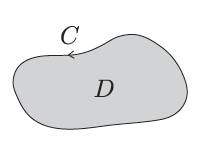
\includegraphics[height=25mm, width=30mm]{green.jpg}
\end{center}
\end{figure}

 \begin{tcolorbox}[
    colback = white,
    colframe = green!35!black,
    fonttitle = \bfseries,
    breakable = true]
    \begin{thm}[グリーンの定理]
$D$を有界閉領域とし$P(x,y),Q(x,y)$を$D$上の$C^1$級関数とすると
 $$
\int_{\partial D} P(x,y)dx + Q(x,y)dy
=
\iint_{D}\left(\pdrv{Q}{x} -\pdrv{P}{y}\right) dxdy\text{\,\,が成り立つ.} 
  $$
 $$
\text{特に}
\Area(D)=\iint_{D}dxdy = \int_{C}xdy=\int_{C}-ydx \text{\,\,が成り立つ.} 
 $$
 \end{thm}
 \end{tcolorbox}
 
 \begin{exa}
  $$
\begin{array}{ccccc}
C: &[0,2\pi] & \rightarrow & \R^2 & \\
&t & \longmapsto &(\cos t , \sin t) &
\end{array}
$$
を滑らかな曲線とする.
線積分$\int_{C}(x^2-y^2)dx-2xydy$を求めよ.

\hspace{-11pt}(解.)普通に計算すると, 
\begin{align*}
\begin{split}
\int_{C}V(\vec{p}) d\vec{p}  
&= \int_{0}^{2\pi} \left \{(\cos^2 t - \sin^2 t)\drv{x}{t}-(2\sin t \cos t) \drv{y}{t} \right \} dt \\
&=\int_{0}^{2\pi} \left \{ -\cos^2 t \sin t + \sin^3 t -2\sin t \cos^2 t  \right\}dt
= \text{(計算略)}
= 0
\end{split}
\end{align*}

グリーンの定理を使う方法は以下のようになる. 
$C$で囲まれた領域$D$とすると, $D$は原点中心の半径1の円である.
$ P(x,y)=x^2-y^2,  Q(x,y)=-2xy$とおくと, グリーンの定理の仮定を満たす. 
$$
\pdrv{Q}{x}=\pdrv{(-2xy)}{x}=-2y, \text{\,\,} \pdrv{P}{y}=\pdrv{(x^2-y^2)}{y}=-2y \text{\,\,であるため, }
$$
$$
\int_{C}(x^2-y^2)dx-2xydy =\iint_{D}\left(\pdrv{v}{x} - \pdrv{u}{y} \right)dxdy = \iint_{D}\left(-2y + 2y \right)dxdy =0.
$$
\end{exa}

\begin{exa}
$a,b$を正の数として, 楕円$D$を下で定める.
$$D = \left\{ (x,y) \in \R^2 : \frac{x^2}{a^2}+\frac{y^2}{b^2} \leqq 1 \right\}
=\left\{ (x,y) \in \R^2 :  -a \leqq x \leqq a, -b\sqrt{1-\frac{x^2}{a^2}} \leqq y \leqq b\sqrt{1-\frac{x^2}{a^2}} \right\}.
$$
$D$の面積$\Area(D)$を求めよ.

\hspace{-11pt}(解.)普通に計算すると, 
\begin{align*}
\begin{split}
\Area(D)=\int_{D}dxdy
= \int_{-a}^{a} \left( b\sqrt{1-\frac{x^2}{a^2}}-(-b)\sqrt{1-\frac{x^2}{a^2}}\right) dx =\int_{-a}^{a} 2 b\sqrt{1-\frac{x^2}{a^2}} dx =\text{(計算略)} = \pi ab.
\end{split}
\end{align*}

グリーンの定理を使うと以下の通りになる.
  $$
\begin{array}{ccccc}
C: &[0,2\pi] & \rightarrow & \R^2 & \\
&t & \longmapsto &(a \cos t, b \sin t)&
\end{array}
$$
とおくと, $C = \partial D$となる.  よってグリーンの定理が使えて, $\drv{y}{t} = b \cos t$のため, 
$$
\Area(D)=\int_{C}xdy=\int_{0}^{2\pi} a \cos t \drv{y}{t} dt
= \int_{0}^{2\pi} ab \cos^2 t  dt = \pi ab \text{となる.}
$$
\end{exa}



\subsection{曲線の長さ  (三宅先生の本, 3.4の内容)}
 \begin{tcolorbox}[
    colback = white,
    colframe = green!35!black,
    fonttitle = \bfseries,
    breakable = true]
    \begin{dfn}
    \begin{comment}
 %   \text{}\begin{itemize}\item 
%関数 $\vec{p}(t)$ を次で定める.
$$
\begin{array}{ccccc}
C: &[a,b] & \rightarrow & \R^2 & \\
&t & \longmapsto &(x(t), y(t))&
\end{array}
$$
が \underline{滑らかな曲線}とは次の2条件を満たすこと.
\begin{itemize}
    \setlength{\parskip}{0cm} 
  \setlength{\itemsep}{0cm} 
\item $x(t),y(t)$共に$[a,b]$上の$C^1$級関数.
\item 任意の$t \in (a,b)$について, 速度ベクトル$ (x'(t), y'(t))\neq  (0,0)$である.
\end{itemize}
%\item \underline{曲線$C: \vec{p}(t) (a \leqq t \leqq b)$が区分的に滑らかな曲線}とは滑らかな曲線を端点でつないだもの.\end{itemize}
\end{comment}


滑らかな曲線$C$に関してその長さを
$$
l(C) = \int_{a}^{b} \sqrt{(x'(t))^2 + (y'(t))^2} dt \text{\,\,\, とする.}
$$
     \end{dfn}
 \end{tcolorbox}
 
  \begin{tcolorbox}[
    colback = white,
    colframe = green!35!black,
    fonttitle = \bfseries,
    breakable = true]
    \begin{thm}
$f(x)$を$[a,b]$上の$C^1$級関数とする. このとき$y=f(x)$のグラフ$C=\{ (x, f(x))\,\,| \,\, a \leqq x \leqq b\}$の長さは
$$
l(C) = \int_{a}^{b} \sqrt{1 + (f'(x))^2} dx \text{\,\,\, である.}
$$
     \end{thm}
 \end{tcolorbox}
 
 \begin{exa}
 放物線$y=x^2 (0 \leqq x \leqq 1)$のグラフの長さを求めよ.
 
\hspace{-18pt} (答.) $f(x) = x^2$とすると$f'(x) = 2x$のため, 曲線の長さは\begin{align*}
\begin{split}
\int_{0}^{1} \sqrt{1 + (2x)^2} dx &= 
\int_{0}^{1} \sqrt{1 +4x^2} dx = 
\frac{1}{2}\int_{0}^{2} \sqrt{1 +t^2} dt \\
&= \frac{1}{4}\left[ t\sqrt{t^2 + 1} + \log \Bigl| t + \sqrt{t^2 + 1 }\Bigr| \right]^{2}_{0} \\
&= \frac{1}{4} \left(2 \sqrt{5} + \log (2 + \sqrt{5})\right)
\end{split}
\end{align*}
 \end{exa}

  \begin{tcolorbox}[
    colback = white,
    colframe = green!35!black,
    fonttitle = \bfseries,
    breakable = true]
    \begin{thm}
$[\alpha,\beta]$上の$C^1$級関数$f( \theta )$を用いて, 曲線$C$が
$$
\begin{array}{ccccc}
C: &[\alpha, \beta] & \rightarrow & \R^2 & \\
&\theta & \longmapsto &(f(\theta) \cos \theta, f(\theta) \sin \theta)&
\end{array}
$$
%$$C: (x(\theta), y(\theta)) = (f(\theta) \cos \theta, f(\theta) \sin \theta)$$
と表されているとき, $C$の長さは
$$
 \int_{\alpha}^{\beta} \sqrt{(f(\theta))^2 + (f'(\theta))^2} d\theta \text{\,\,\, である.}
$$
     \end{thm}
 \end{tcolorbox}
 
 \begin{exa}
(アルキメデスの螺旋)
正の実数$a , \alpha $について
$$
\begin{array}{ccccc}
C: &[0,\alpha] & \rightarrow & \R^2 & \\
&\theta & \longmapsto &(a \theta \cos \theta ,  a \theta \sin \theta)&
\end{array}
$$
 とする. 曲線$C$の長さを求めよ.
 
\hspace{-18pt} (答.) $f(\theta) = a \theta$とすると$f'(\theta) = a$のため, 曲線の長さは\begin{align*}
\begin{split}
\int_{0}^{\alpha} \sqrt{a^2 + (a \theta)^2} d\theta = 
a \int_{0}^{\alpha} \sqrt{1+ (\theta)^2} d\theta = 
\frac{a}{2}\left(\alpha\sqrt{\alpha^2 + 1} + \log (\alpha + \sqrt{\alpha^2 + 1})\right)
\end{split}
\end{align*}
 \end{exa}


\newpage
\section{演習問題} 

\begin{comment}

$\bullet$ \ref{kihonteiri}節の問題 正の自然数$n,x \in \N$について
$$S_{n}(x) = \sum_{k=1}^{n}\frac{1}{k^x}$$
とおく. 次の問いに答えよ.
\begin{enumerate}
\item $\lim_{n \rightarrow \infty} S_{n}(1)$は発散することを示せ.
\item $\lim_{n \rightarrow \infty} S_{n}(2)$は収束することを示せ.
\end{enumerate}
ちなみに下の等式が成り立つことが知られている.
\begin{align*}
\begin{split}
\frac{\pi^2}{6} &= \lim_{n \rightarrow \infty} S_{n}(2) = 1 + \frac{1}{4}+ \frac{1}{9}+ \frac{1}{16}+ \frac{1}{25}+
\cdots  \\
\frac{\pi^4}{90} &= \lim_{n \rightarrow \infty} S_{n}(4) = 1 + \frac{1}{2^4}+ \frac{1}{3^4}+ \frac{1}{4^4}+ \frac{1}{5^4}+
\cdots  \\
\frac{\pi^6}{945} &= \lim_{n \rightarrow \infty} S_{n}(6) = 1 + \frac{1}{2^6}+ \frac{1}{3^6}+ \frac{1}{4^6}+ \frac{1}{5^6}+
\cdots  \\
\end{split}
\end{align*}
\end{comment}

%\hspace{-18pt}
$\bullet$\ref{1_2}節の問題
%演習問題の解答は授業の黒板にあります.
\begin{enumerate}
    \setlength{\parskip}{0cm} 
  \setlength{\itemsep}{0cm} 
\item 不定積分$\int x\log x \,dx$を求めよ.
%\item 不定積分$\int \log x \,dx$を求めよ
\item 定積分$\int_{0}^{1} x  e^{2x} \,dx$を求めよ.
\end{enumerate}

\hspace{-18pt}$\bullet$\ref{1_3}節の問題
\hspace{11pt}不定積分$\int \frac{x^2}{x^2 - x - 6}dx$を求めよ.

\hspace{-18pt}$\bullet$\ref{2_2}節の問題
 $D=\{ (x,y) \in \R^2 : 0 \leqq y, \text{\,} 0 \leqq x-y, \text{\,} x+y \leqq 2\}$とする.
重積分$\iint_{D} (x^2-y^2)dxdy$の値を求めよ.

\hspace{-18pt}$\bullet$\ref{2_3}節の問題
 $D=\{ (x,y) \in \R^2 : 0 \leqq x, \text{\,}  0 \leqq y,\text{\,} \sqrt{x} + \sqrt{y} \leqq 1\}$とする.
重積分$\iint_{D} x^2dxdy$の値を求めよ.

\hspace{-18pt}$\bullet$\ref{2_4}節の問題
\begin{enumerate}
    \setlength{\parskip}{0cm} 
  \setlength{\itemsep}{0cm} 
\item $a>0$とする. 円柱$x^2 + y^2 \leqq a^2$と球$x^2 + y^2 + z^2 \leqq a^2$の共通部分の体積を求めよ.
\item$ V = \{ (x,y,z) \in \R^3 | x^2 + y^2 + z^2 \leqq 1\}$とする. 重積分
$$
\iiint_{V} x dxdydz
$$
の値を求めよ.
\end{enumerate}

\hspace{-18pt}$\bullet$\ref{3_1}節の問題 
\hspace{11pt}$p$を実数とし$f(x) = x^p \log x$とする.
\begin{enumerate}
    \setlength{\parskip}{0cm} 
  \setlength{\itemsep}{0cm} 
%\item[] $p$を実数とし$f(x) = x^p \log x$とする. 
\item $p< -1$ならば広義積分$\int_{1}^{\infty} f(x) dx$は収束することを示せ.
\item $p\geqq -1$ならば広義積分$\int_{1}^{\infty} f(x) dx$は発散することを示せ.
\end{enumerate}

 
 \end{document}
 

 
